\documentclass{article}
\usepackage{graphics}
\usepackage{fancyhdr}
\usepackage{url}
\usepackage{helvet}
\usepackage{graphicx}
\usepackage{setspace}
\usepackage[margin=1.25in]{geometry}
\usepackage{textcomp}
\usepackage{hyperref}
\usepackage[utf8]{inputenc}
\usepackage{cite}
\usepackage{microtype}
\graphicspath{ {images1/} }


\DisableLigatures{encoding = *, family = * }

\newcommand{\name}{Renan Greca}
\newcommand{\website}{www.renangreca.com}
\newcommand{\email}{renangreca@gmail.com}

\usepackage[font=small,labelfont=bf,labelsep=space]{caption}
\captionsetup{%
  figurename=fig.,
  tablename=tab.
}

\bibliographystyle{alpha}  

\begin{document}

%\fontfamily{phv}\selectfont
\pagestyle{fancy}
\lhead{\name}
\chead{}
\rhead{\email}
\lfoot{}
\cfoot{\thepage}
\rfoot{}

\inputencoding{latin1}

\begin{center}
    \Large
    \textbf{} \\
    \textit{Renan Greca} \\
    %\coursetitle - Research Paper\\
    \small
\end{center}

\large
\doublespacing

\section{Introduction}



\section{Complex Networks}
Complex networks can describe many systems which are observed in nature and society, such as computer networks, food chains, protein structures, etc. \cite{newmannetworks}
They are frequently divided into four categories: technological networks, social networks, information networks, and biological networks.

\textbf{/*********}
Many networks have some concept of trust.
In peer-to-peer information networks, nodes have complete control over their own data \cite{vernize2015malicious}, so other nodes must trust that the data they receive is the one they requested.
Trust in the context of social networks will be elaborated in this section, while technological networks will be further examined in the next section.
\textbf{*********/}

\subsection{Trust in Social Networks}
In a traditional social network, it is simple to perceive how trust is relevant and how it works, since trust relationships between people (friends, relatives, colleagues, etc.) are used on a daily basis to make decisions.
When adapted to a digital environment, these social relationships can be used to automatically increase the relevance of certain information.
For instance, upon reading an online review for a certain product, a user will be more likely to accept the review's conclusion if it was written by a close friend than if it were written by a stranger.
Furthermore, if the review was written by a person who the user knows to be malicious or uninformed, its contents will be even less relevant.
In short, trust is a way of estimating how much a certain recommendation will lead to a positive outcome. \cite{golbeck2006inferring}

Social networks also have the property of carrying trust from one relationship to another:
information shared by a close friend of a person might be considered almost as trustworthy as some collected by the person him or herself.
Therefore, it is possible to model social trust relationships as a graph, in which nodes represent people and edges represent a certain degree of trust.
Friends of friends \cite{boissevain1974friends} might not have very high trust values, but could still be considered more trustworthy than the average stranger.
This property is similar, but not identical, to transitivity, since trust is diminished for each extra step an origin node needs to take to reach it (a friend of a friend is more trustworthy than a stranger, but is less than a direct friend).

Social networks also have the trait of being mostly static.
Although friendships are formed and ended frequently, those connections do not disrupt the general shape of the network.
In fact, the ending of a friendship might indicate the presence of a \textit{negative} trust relationship between two people.
Such negative information can be useful in digital social networks since that data might not be available.
% \textemdash for example, on Facebook, people are usually only connected if there is a positive relationship between them.

\subsection{Existing trust models for Complex Networks}

%[description of complex networks]

%[examples of complex networks]

%[details of how trust can be established in complex networks]

%[existing trust models applied in complex networks]

%[small world phenomenon]

\section{VANETs}

%[description of VANETs]

%With the increasing feasibility of smart and autonomous vehicles, the study of Vehicular Ad-hoc Networks (VANETs) is ever more important \textbf{[CITE]}.
The prospect of autonomous vehicles makes the study of Vehicular Ad-hoc Networks (VANETs) important.
However, it will still take many years before completely autonomous vehicles are the norm and, until then, VANETs can be a valuable tool to help drivers reduce travel times and diminish the risk of collisions.
The vehicles' on-board computers can aid drivers to increase safety and reduce traffic, but data needs to be shared among the various vehicles in the network.
Such data includes location, speed and destination, which neighboring vehicles can use to adjust their trajectory and increase their own efficiency.
% By allowing vehicles to share their locations, speeds, and destinations with each other, traffic can become more stable and predictable.
Thousands of people die each year due to traffic accidents, many of which could have been avoided if vehicles were smarter and able to provide important alerts both to their drivers and to neighboring vehicles.

\begin{figure}[h]
    \centering
    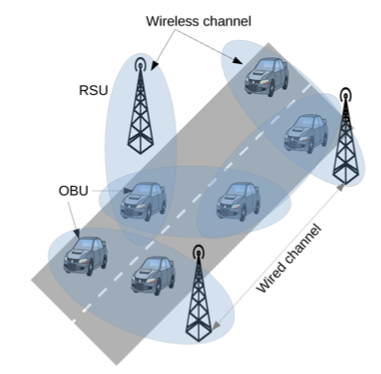
\includegraphics[width=0.5\textwidth]{images/vanet.png}
    \caption{Basic elements of a VANET: OBUs and RSUs. \cite{saini2015close}}
    \label{fig:vanet}
\end{figure}

Current efforts to make VANETs viable in cities are centered around the IEEE 802.11p standard, also called Wireless Access in Vehicular Environments (WAVE) \cite{jiang2008ieee}.
Amongst other aspects of the wireless technology, the WAVE standard describes two types of nodes for vehicular networks: on-board units (OBUs) and road-side units (RSUs).
On-board units are computers placed within each vehicle which monitor the vehicle's data and are able to communicate with other nodes using wireless signals.
Road-side units are placed in static locations near roads; they may also have wired interfaces with other RSUs and the Internet, so it is possible to use them as anchor points for Internet access for passing vehicles.

%[description of trust in context of VANETs]

\subsection{Trust in VANETs}

Like in other types of networks, the proper functioning of a VANET depends on the reliability of the vehicles (nodes) of the network.
If one node is malicious or faulty, it can spread incorrect data that may compromise the utility of the VANET.
Once the concept of VANETs was established, researchers have been attempting to predict ways in which malicious users might use the network to their advantage.
Examples include triggering false alarms about inexistent accidents, lying about the average speed in one road to make it less desirable for others, and falsifying geolocation data to exploit location-based routing algorithms. Therefore, the concept of trust must be established in the vehicular network context, allowing for nodes to judge the validity of information transmitted by others and share those conclusions with other nodes.

There is an important distinction between a malicious node and a faulty one; both of them may be sharing false data, but for different reasons and with different consequences.
For example, a malicious node may lie about its location in order to make routing protocols use it \cite{leinmuller2005influence}, while a faulty GPS module may cause an accident because its position data was incorrect.
However, that distinction can be hard to make, because a close inspection is necessary to determine whether the incorrect data is erratic or deliberate.
Since both types of nodes are problematic to the proper functioning of a network, malicious and faulty nodes can be treated as the same in a trust model.

%\textbf{/*********}
%Trust can be a related, yet distinct, issue to cryptography and authentication in vehicular networks.
%Many studies propose the use of a PKI (Public Key Infrastructure) to guarantee legitimate identities for nodes, although this solution requires, by definition, a certifying authority to manage and distribute public keys.
%VANETs must be able to function in a completely independent fashion, regardless of the amount of active nodes in a given region, and without relying on a centralized service.
%Both trust and authentication must work together to provide an adequate solution for VANETs, since it is difficult to establish trust without means to verify an identity (a malicious node may provide false data about its identity to bypass trust solutions), while a cryptography system requires a pre-existing infrastructure and may add unacceptable latency to high-priority messages.
%\textbf{[moved to chapter 4]}
%\textbf{*********/}

Some solutions use \textit{data-oriented trust} (or \textit{data-centric trust}) \cite{raya2008data}.
Those solutions focus on validating messages instead of entities, and are especially important when dealing with event-based trust.
This is important when vehicles share messages about a specific event, such as a collision, which must be quickly validated by neighbors and distributed to other nodes within a relevant area.
In this scenario, vehicles sharing the same road might be complete strangers to each other, and therefore will not have any trust relationship, so neighboring nodes must decide if a message is true purely by its contents.

On the other hand, when dealing with frequent messages which contain basic information such as geolocation and speed (used for traffic-diminishing solutions), it is too costly to judge each individual message.
Therefore, \textit{entity-based trust} becomes more appealing, since benign nodes can quickly identify a malicious node and isolate it from the network.
These models take advantage of the possibility of nodes meeting more than once and, therefore, being able to form a long-term trust relationship with each other.

%\textbf{/*********}
%In \cite{gerlach2007trust}, the author shows a general framework of how security and trust can be organized in a vehicular network.
%It proposes three layers: a service plane, which contains the core functionalities of the network, such as communication technologies, routing algorithms and the security measures directly related to them (such as cryptography); a middleware plane which handles trust and privacy issues; and the application layer, which contains the applications that will use the other layers' data to make decisions.
%The model shows neatly how security and trust can interact with each other to provide best results.
%\textbf{*********/}

%[malicious and faulty nodes]

%[details of security and safety issues in VANETs that can be diminished by trust]


\subsection{Existing trust models for VANETs}

Several models have been proposed to solve the problem of trust in vehicular networks. 
In this section, some of the most relevant ones will be described, taking into consideration the time in which they were proposed, the advantages they bring and their contributions to later study. 
None of them provide a complete solution, but serve as pieces of a puzzle that is, at the time of writing, still incomplete. 
Some review and/or survey articles have been written on the subject of VANET trust models, such as \cite{zhang2011survey}, \cite{ma2011survey}, \cite{mejri2014survey}, \cite{sengar2016survey}, and \cite{dwivedi2016review}. 

\cite{dotzer2005vars} is one of the earliest examples of VANET trust models, establishing a system called VARS, based on the reputation of nodes and messages throughout the network.
The authors use what they call \textit{opinion piggybacking}, which means that, for each hop between the origin and the destination of an event-related message, the forwarding node will append its opinion of the message's contents.
That opinion is formed using a combination of the forwarding node's own observations of the event, its opinion of the origin node and previous opinions appended to the message.
This trust model works as a way of adding credibility of a message through validation by its sender's peers in a non-centralized fashion.
It combines aspect of data- and entity- based trust, since nodes share their opinion of the data as well as their opinion of the sender. 
One interesting observation is setting higher trust values for certain vehicles based on their familiarity with the region (vehicles that reside in a given city may have more experience with certain types of events than newcomers).
However, opinion piggybacking has its own share of problems.
First, it means that forwarding nodes must be able to access (at least some of) the contents of a message so it can form an opinion on it, diminishing privacy; a malicious forwarding node could even attempt to alter those contents.
Second, using previously appended opinions from other nodes to form a new opinion means that the first nodes to forward the message will have a substantially greater impact over the final opinion than the later ones.
Finally, there is an issue with scalability, since appending new information to a message on each hop may add a significant overhead to the transmission. Additionally, the authors provide little to no experimentation or proof that their approach would be sound in a real-world network.

In \cite{chen2010trust}, the authors propose to evaluate messages utilizing a cluster-based trust model.
By separating nodes into clusters with their geographical neighbors, it is possible to efficiently distribute the evaluation of messages using previously formed opinions.
When a node sends a message, one node in the cluster (the leader) must aggregate the other node's opinions on that message.
Afterward, the message is only forwarded to another cluster if that aggregate opinion is above a certain threshold; furthermore, nodes that receive the message will only act upon it if the overall trust on it is above another threshold, which can be different according to the nature of the message.
However, it is unclear how the model behaves when the network is too sparse to form relevant clusters, neither do the authors inform how the aforementioned thresholds are decided.
Furthermore, if the cluster leader itself is malicious, all the information from that cluster becomes untrustworthy. 
The model takes into consideration role-based trust (i.e. static trust of pre-authenticated vehicles such as police units) and experience-based trust, which is calculated using knowledge of the outcomes related to previous messages.

The authors of \cite{huang2014social} take special note of two characteristics from social networks that can also be found in many VANET trust models: \textit{information cascading} and \textit{oversampling}.
That is, information reported by a number of original nodes (i.e. the ones that witnessed an event) may be diluted as nodes that forward it append their own opinions on the matter.
An algorithm is proposed to diminish that effect by assigning higher weights to the opinions of origin nodes and lower weights  to others.
However, the authors conclude that the optimal scenario is to assign no weight at all to forwarding nodes, therefore allowing each node to form an opinion based only on the original nodes' reports.
Furthermore, the authors are quick to dismiss the validity of [node-based reputation, check proper name], instead opting for a pure message-based approach.
Since their model is based only on events, it also does not consider the usefulness of trust in more mundane cases such as the frequent sharing of location and speed among vehicles.

The trust model in \cite{park2011long} takes advantage of daily commutes.
In this article, the focus is on the early stages of VANETs, in which a very small percentage of vehicles will be equipped with OBUs.
To make trust viable in such a scenario, the authors rely on RSUs to store reputation information from passing vehicles.
Each vehicle must have an ``Agent RSU'', which will be tasked with sharing that vehicle's trust data to other vehicles and RSUs as well as keeping the data updated when the vehicle is near it once again.
To make this viable, the properties of daily commutes are used: it is assumed the vehicle will be near that RSU with reasonable frequency because it is located within the driver's home-to-work route.
The main problem with this model is that it relies on the presence of frequent RSUs, which might not always be viable.
It also does not make it clear what should happen when a vehicle stops using a route or does not have a daily predictable path (it does, however, handle occasions in which a vehicle chooses an alternate route or is absent for some days such as weekends and holidays).

%[data-oriented vs entity-oriented trust]

\section{Complex network trust model applied in VANETs}

Several of the aforementioned articles state that vehicular networks are, by definition, ephemeral.
That is, the likelihood of two nodes meeting each other twice is too low to be relevant.
In this work, it is argued that such claims are not entirely true.
It stands to reason that, throughout the course of several days, many drivers will take similar routes at similar times of day (e.g. to commute to work) and, therefore, their vehicles will be in similar locations each day.
Additionally, many cities rely on main roads to serve as backbones to their traffic, meaning there is a high density of vehicles on those roads during rush hours.
Since that is true for a notable percentage of a city's fleet, we can also assume that those vehicles may frequently encounter each other during their commute.
While two vehicles that share a commute route may not be direct neighbors every day, they will likely be relatively close to each other, meaning few hops separate them in the ad-hoc network.

%\textbf{[WORKING DAY MOBILITY MODEL]}

In \cite{da2013effective}, \cite{cunha2014vehicular}, and \cite{cunha2014possible}, the authors attempt to find features usually attributed to social networks in vehicular networks.
By using a data set from Zurich, they show that some metrics, such as clustering coefficient and number of encounters, have peaks during the rush hours.
They do not, however, present data regarding specific pairs of nodes.
%[Should we propose to show this information in our work?]

Additionally, certain pairs of vehicles are bound to be within communication range of each other nearly every day.
Examples of these include vehicles whose owners are drivers or coworkers.
Such vehicles' trust relationship should become steady over time and, in the case of positive trust, they can use each other's information to learn more about other nodes in the network.

Regardless of these properties of commuting vehicles, the probability of two specific vehicles meeting each other more than once, in given time, tends to 1.
So it is also reasonable to assume that two vehicles, whose drivers reside in the same city, over a long period of time (e.g. one year) may meet each other more than once.
However, if they only meet rarely, their trust opinions about each other may not be very useful.

Most cities also have one or more types of mass transit systems (buses or trains).
Those vehicles can also be part of a VANET and communicate with private cars.
Buses share the same roads as cars, but instead of having specific destinations, they travel a predefined route during the whole day, usually tied to a tight schedule.
Trains travel on rails, so their contact with cars is less frequent, but it can also happen on railroad crossings; they travel long distances in relatively short amount of time, which helps the dissemination of data in a VANET.
In the same way that cars have a high probability of meeting more than once during their commutes, it is also very likely that they will meet the same buses and/or trains frequently.

Another way of applying trust models from social networks to VANETs would be to take into account the relationships between drivers.
If a neighboring vehicle happens to be driven by a close friend or relative, there is reason to believe that it is not a malicious node in the network.
That might not always be the case, since there may be malicious hackers controlling the node and its driver is oblivious to it.
In any case, this approach is not covered in this work.

While certification of identity is an issue in vehicular network, this work will not address it.
There are studies focusing on node identification in VANETs (that is, making sure a node is who it claims to be), in particular through the use of a Public Key Infrastructure (PKI) \cite{wasef2010complementing} 
\cite{kumar2015intelligent}.
One study even proposes that such identities must be refreshed with a certain frequency to maintain the privacy of each node \cite{golle2004detecting}.
Although it is important that nodes are not able to lie about identity and are able to maintain their privacy, nodes having valid identities that are persistent over time is a prerequisite for the model proposed here.

\subsection{Working Day Movement Model}

To make use of the above properties, it is important to choose a mobility model that properly represents the way vehicles move on a daily basis in the real world.
Therefore, the Working Day Movement Model \cite{ekman2008working} will be used.
The model, developed for used in Delay-Tolerant Network (DTN) simulations, includes many of the features that will be necessary to simulate the daily movement of a vehicular network.

As the name implies, the Working Day model abstracts people's movement from their homes to their offices and back.
Each node has a home and a workplace and they need to travel back and forth between those locations on a daily basis.
Occasionally, nodes can also go to other locations for leisure.
Most VANET trust models use the Random Waypoint mobility model, i.e., each node has an origin point, chooses a random location, gets to that location, then chooses another random location and goes there, and so forth.
While this model is efficient for testing trust protocols, it doesn't truly represent vehicle mobility in the real world.
As mentioned above, many drivers have routes they travel on daily, so the Working Day model is a more accurate representation, although it represents the mobility of humans instead of vehicle and requires some adjustments, which will be listed later in this section.

The model proposed by the authors makes use of several other models for specific tasks.
The main mobility model defines nodes and gives them their destinations.
Within it, five other models are used:
\begin{enumerate}
\item 
The \textbf{home activity submodel} describes what nodes do at night, within their homes.
No movement is modeled.
Nodes can be relatives or neighbors, and therefore share the same home.
\item 
The \textbf{office activity submodel} describes the nodes' routines within their offices.
Nodes can go to other locations within the office (such as meeting rooms) and such movement is modeled.
Nodes with share the same office are coworkers.
\item 
The \textbf{evening activity submodel} is responsible for mobility outside the nodes' standard routine. 
They can meet at certain locations (such as restaurants) and spend a few hours gathered with friends.
\item
The \textbf{transport submodel} shows how nodes move around the city.
It includes another tier of submodels, responsible for modeling three different types of transportation: walking, driving, and riding a bus.
Nodes which own a car always use it, while the others can decide to walk or ride a bus depending on the distance between the origin and destination and the available bus stops.
The walking and driving submodels represent similar types of movement, although at different speeds, while the bus submodel follows cyclical routes and can take or deliver passengers at bus stops.
\item
The \textbf{map} represents the city in which the simulation runs.
Its streets constrain the movement of nodes and all homes and offices must be within the map boundaries.
The map can be divided into districts, which increases what the authors define as \textit{locality}.
In the simulation parameters, the number of nodes which reside and work within the same district can be chosen, which means those nodes will rarely leave the district.
Nodes which reside and work in different districts serve to connect the network with their commutes.
\end{enumerate}

By thinking of these submodels for vehicles instead of people, it can become apparent how the frequency and length of encounters between nodes are similar in both instances.
If two vehicles belong to family members or neighbors, they will likely spend most of the night within communication distance, while coworkers' cars spend the office hours close by.
Cars can also meet each other frequently if their drivers go out with friends.
In the vehicular case, there is the added layer of encounters: cars can communicate frequently with buses and other cars that take the same route daily, although the drivers are likely complete strangers.

In the original article, nodes are devices (such as smartphones) being carried by humans.
Therefore, the Working Day model represents not only people's movements inside their cars, but also within their offices, walking on foot, or riding a bus.
To adapt it to a VANET environment, changes need to be made to their definition of node, since they now represent vehicles instead of people. Some of those changes are as follows:
\begin{enumerate}
\item
The office activity submodel no longer needs to model movement within the office and can be identical to the home submodel.
In both these submodels, a node can move a small amount once after reaching the office or home, to simulate parking.
This can be done using the Working Day model's parameters.
\item
The walking submodel needs to be disabled, since all nodes will be either cars or buses.
\item
The bus submodel needs to be changed so that each bus is one node in the network, which follows a predefined route with bus stops.
In the original model, each bus could carry several nodes, but this is no longer necessary.
\end{enumerate}
Other necessary changes might become apparent during the development of the study.

One important topic raised in the Working Day movement model article is the use of two metrics: \textit{inter-contact times} and \textit{contact duration}.
The choice of this movement model for tests is more strongly related to inter-contact times, i.e. how much time it takes for two nodes to meet again.
On the other hand, the contact duration is how long each meeting lasts.
For the reasons explained earlier in this section, relatively short inter-contact times is important for the proposed trust model.
Contact duration time is an important metric to measure how much data can be exchanged during each encounter, although taking it into consideration might add excessive complexity to the model.

\section{Proposal}

As described above, properties derived from social networks will be used to adapt a trust model developed for static complex networks to dynamic ones.
The basis of the proposed trust model is \cite{vernize2015malicious}.
This article presents a malicious node identification scheme based on strongly connected components and graph coloring.

First, a graph $G$ is separated into components so that each component contains only nodes that trust each other (in other words, any distrust in a relationship between two nodes is enough to separate them into different components).
Then, on the supergraph $T$ whose nodes are $G$'s components, a graph coloring algorithm is used.
The color with the most nodes in $T$ is deemed correct, while the others are deemed incorrect.
This means the correct color contains only trustworthy nodes, and the others contain nodes of dubious trustworthiness.

\subsection{Changes}
While the algorithm described above works well for static graphs, some important modifications will have to be made to accommodate dynamic graphs.
The main changes planned are described below.

\subsubsection{Trust graph}
The original work's scope does not include the generation of the trust graph, as it is a parameter to the algorithm.
In dynamic graphs, trust relationships change over time, so how those changes affect our trust model have to be taken into consideration.
This includes not only the full figure of the graph, but also each node's views on its neighbors.

\subsubsection{Strongly connected components}
Strongly connected components, or components in which all nodes have positive trust relationships with each other, are somewhat different in dynamic graphs.
As nodes enter, leave, or change locations in the network, the components will change accordingly.
Therefore, our algorithm will have to work using ``snapshots'' of the graph, meaning each measurement will be valid for a specific timestamp.
In a later step, it might be useful to take into consideration how specific nodes may change over several snapshots.

\subsubsection{Graph knowledge}
In the original paper, the malicious nodes are identified by a central entity with access to all nodes' trust values.
Not only does our work plan to decentralize this procedure, having complete knowledge of the graph is unfeasible in large-scale dynamic networks such as VANETs.
Therefore, our algorithm needs to work using only a partial understanding of the network.
For this to be viable, each node will likely have to gather information not only from its views on its neighbors, but also from its neighbor's views and so forth.

The authors of \cite{patwardhan2006data} provide important observations regarding the collection of data from local conditions.
Most crucially, they mention how the quality of information is higher when the origin of such information is close to the destination node.
That is, data collected by the node's own sensors have the highest quality, which diminishes as information starts to come from neighbors, neighbors of neighbors and so forth.
They adopt a broadcast model in which RSUs send data about its surroundings and OBUs capture the information.
The trust model proposed here might use a similar broadcast model, although adapted so all nodes are vehicles (OBUs).

\subsubsection{Binary trust}
A model using binary trust is one in which trust values can only be 0 or 1.
If node $A$ positively trusts node $B$, the value of the edge $A\rightarrow B$ is 1.
If it does not trust $B$, or is unsure, the value is 0.
Such a scheme makes sense in a static graph but, in a dynamic one, it is interesting to have a range of possible trust values.

Since nodes will interact with each other occasionally and might learn information from other nodes, a range such as $[0,1]$ is useful to express how one trust value can change over time.
As one node learns more about another, the value can grow or diminish and, once it goes above or below a certain threshold, the neighboring node can be deemed trustworthy or not.

\subsubsection{Datasets}
The datasets used for experimentation must be changed accordingly.
Instead of using data gathered from social networks, we will need to use dynamic network datasets, such as traffic information for cities.

%[how we plan on adapting the previous works]

%[what do we expect to change]

%[what do we expect to be the challenges]

%[scenario context (speed, density, etc)]



\bibliography{qualification}
 
\end{document}